% \documentclass[10pt, letterpaper]{article}
\documentclass[10pt,twocolumn,letterpaper]{article}
% \usepackage[a4paper, total={6in, 8in}]{geometry}
\usepackage{cvpr}
\usepackage{times}
\usepackage{epsfig}
\usepackage{graphicx}
\usepackage{amsmath}
\usepackage{amssymb}
\usepackage{enumitem}
\usepackage{url}
\usepackage{mathrsfs}
\usepackage{float}
\usepackage{amsfonts,nicefrac,mathtools,bbm,color}
\usepackage{verbatim}

\newcommand{\real}{\mathbb{R}}

\newcommand{\bsx}{\boldsymbol{x}}

\newcommand{\e}{\mathbb{E}}
\newcommand{\var}{\mathrm{var}}

\newcommand{\rct}{\mathcal{R}}
\newcommand{\odb}{\mathcal{O}}

\newcommand{\err}{\varepsilon}

\renewcommand{\le}{\leqslant}
\renewcommand{\ge}{\geqslant}

\newcommand{\tran}{\mathsf{T}}

\newcommand{\simiid}{\stackrel{\mathrm{iid}}\sim}

\newcommand{\rd}{\,\mathrm d}

% Specialized notation. 
% Small roman subscripts are more readable than smal italic ones.

\renewcommand{\k}{\mathrm{k}}
\renewcommand{\r}{\mathrm{r}}
\newcommand{\s}{\mathrm{s}}
\renewcommand{\o}{\mathrm{o}}

\newcommand{\rk}{\mathrm{rk}}
\newcommand{\rkt}{\mathrm{rkt}}
\newcommand{\rkc}{\mathrm{rkc}}
\newcommand{\rt}{\mathrm{rt}}
\newcommand{\rc}{\mathrm{rc}}

\newcommand{\ok}{\mathrm{ok}}
\newcommand{\okt}{\mathrm{okt}}
\newcommand{\okc}{\mathrm{okc}}

\newcommand{\ot}{\mathrm{ot}}
\newcommand{\oc}{\mathrm{oc}}

\newcommand{\sk}{\mathrm{sk}}
\newcommand{\skt}{\mathrm{skt}}
\newcommand{\skc}{\mathrm{skc}}

\newcommand{\st}{\mathrm{st}}
\renewcommand{\sc}{\mathrm{sc}}


\newcommand{\nr}{n_{\r}}
\newcommand{\nrk}{n_{\rk}}
\newcommand{\nrkt}{n_{\rkt}}
\newcommand{\nrkc}{n_{\rkc}}

\newcommand{\nrt}{n_{\rt}}
\newcommand{\nrc}{n_{\rc}}


\newcommand{\no}{n_{\o}}
\newcommand{\nok}{n_{\ok}}
\newcommand{\nokt}{n_{\okt}}
\newcommand{\nokc}{n_{\okc}}

\newcommand{\fr}{f_{\r}}
\newcommand{\fo}{f_{\o}}

\newcommand{\byr}{\bar Y_{\r}}
\newcommand{\byrk}{\bar Y_{\rk}}
\newcommand{\byrkt}{\bar Y_{\rkt}}
\newcommand{\byrkc}{\bar Y_{\rkc}}

\newcommand{\byrt}{\bar Y_{\rt}}
\newcommand{\byrc}{\bar Y_{\rc}}

\newcommand{\byo}{\bar Y_{\o}}
\newcommand{\byok}{\bar Y_{\ok}}
\newcommand{\byokt}{\bar Y_{\okt}}
\newcommand{\byokc}{\bar Y_{\okc}}

% Include other packages here, before hyperref.

% If you comment hyperref and then uncomment it, you should delete
% egpaper.aux before re-running latex.  (Or just hit 'q' on the first latex
% run, let it finish, and you should be clear).
\usepackage[breaklinks=true,bookmarks=false]{hyperref}

\cvprfinalcopy % *** Uncomment this line for the final submission

\def\httilde{\mbox{\tt\raisebox{-.5ex}{\symbol{126}}}}

% Pages are numbered in submission mode, and unnumbered in camera-ready
%\ifcvprfinal\pagestyle{empty}\fi
\setcounter{page}{1}
\begin{document}

%%%%%%%%% TITLE
\title{Using Poisson Binomial GLMs to Reveal Voter Preferences}

\author{Evan Rosenman\\
Stanford University\\
{\tt\small rosenman@stanford.edu}
% For a paper whose authors are all at the same institution,
% omit the following lines up until the closing ``}''.
% Additional authors and addresses can be added with ``\and'',
% just like the second author.
% To save space, use either the email address or home page, not both
\and
Nitin Viswanathan\\
Stanford University\\
{\tt\small nviswana@stanford.edu}
}

\maketitle
%\thispagestyle{empty}

%%%%%%%%% ABSTRACT
% \begin{abstract}
% TODO
% \end{abstract}

%%%%%%%%% BODY TEXT

\section{Abstract}

\section{Introduction}
Political organizations seek to build voting models to explain individual voter preferences, as this information is vital for voter targeting. For example, they want to identify swing voters and split ticket voters (who voted for candidates across multiple political parties) to focus outreach efforts for future elections.

In the US, voting data indicating how many votes every candidate receives is available at the precinct level, but the most granular data – who voted for which candidate – is private. As a result, political groups are forced to rely on polling data to perform analysis at the individual voter level. However, polling has not been correct in several recent elections, most notably the 2016 presidential election. Polling data can not only be unreliable but it is also incomplete, as voters are not obligated to express their true preferences and the majority of voters will not participate in polls. We develop individual voter models based off of publicly available precinct-level voting data.

Using precinct-level data, we develop a new type of GLM to explain individual voter behavior in Pennsylvania for the 2016 presidential election. We focus on predicting votes for both Hillary Clinton and Donald Trump in the state of Pennsylvania as it was a key swing state that went in favor of Donald Trump in the 2016 presidential election. Trump's margin of victory was very slim at only 44,292 votes, only 0.72\% more than Clinton's \cite{NYT}. Precinct-level election results are the most granular results available; for reference there are about 9,000 precincts total in Pennsylvania \cite{NYT}. 

We formulate the problem using a Poisson binomial generalized linear model, which has not to our knowledge been done before in other literature. We then minimize the negative log-likelihood via batch gradient descent.

Our paper makes two key contributions:
\begin{itemize}[noitemsep]
	\item We develop the math necessary to use and train Poisson binomial GLMs
	\item We apply poission binomial GLMs to the specific task of revealing voter preferences
\end{itemize}

\section{Related Work}
Theoretical work on the Poisson Binomial distribution has focused on computationally tractable ways to estimate its distribution function, often via approximations to other distributions 
\cite{EHM19917, roos1999, chen1974}. Prior research \cite{HONG201341} has identified a closed-form expression for the CDF, which relies on the discrete Fourier Transform. This technique is leveraged in the \texttt{poibin} package \cite{PoibiGithub}, which we use for this project. The application of the Poisson Binomial distribution to the generalized linear model setting has been discussed by Chen and Liu \cite{Poibi}, who propose it for hypothesis testing on the parameter vector for a logistic regression model. 

There is a richer body of literature on our chosen problem: modeling voter preferences in elections. Most of this research separates into two primary methodologies. In the first, researchers are interested in the relationship between voter characteristics and their ballot preferences. To obtain labeled datasets, researchers make use of voter surveys \cite{dubrow2007choosing}, exit polls \cite{carsey1995contextual}, or modeling whether an individual voted (which is public record), rather than her choice of candidate \cite{rusch2013influencing}. They then fit models via simple GLMs, like the multinomial probit or multinomial logit model, which ``represent voter choice as a decision among unordered alternatives (parties, candidates) as a function of chooser (voter) and choice (party/candidate) attributes" \cite{DOW2004107}. 

In the second methodology, researchers are interested in the relationship between candidate characteristics or voting methods and vote outcomes. In these studies \cite{miller1998impact, frisina2008ballot, 10.2307/24371899}, researchers frequently use aggregate vote totals from precincts, counties, or states. Relationships are then uncovered by linear regression techniques, often using some random effects \cite{10.2307/2585758} and modified to include constraints. Closely related to this literature is the approach of popular election prognosticators like FiveThirtyEight \cite{538} to model election outcomes using a mix of polling and demographic data. 

Lastly, the problem of ``learning individual-level associations from aggregate data" \cite{flaxman2015supported} has precedent in more modern machine learning literature \cite{patrini2014almost, kuck2012learning, sun2015message, quadrianto2009estimating}. These papers relate individual-level covariates to aggregate statistics by estimating individual level probabilities; this is frequently done by applying kernels to the covariates and then using a probit or logit link. Their fitting methods, however, rely on Bayesian techniques rather than the asymptotic normality utilized here. In the political setting, Flaxman et al. have used individual-level covariates to analyze the 2012 \cite{flaxman2015supported} and 2016 \cite{flaxman2016understanding} presidential elections, but their approach does not estimate individual-level probabilities but rather uses kernel techniques to relate individual features to aggregate statistics. Thus, we believe our fitting procedure via the normal approximation to the Poisson binomial distribution is novel.

\section{Dataset}

\subsection{Overview}

We combined two disparate datasets for our project. \\

Our dataset of \textbf{Pennsylvania precinct-level election results} contains the total number of votes received by each candidate by precinct in the 2016 presidential election. We obtained this dataset from OpenElections \cite{OpenElections}.

\begin{table*}
\caption{Pennsylvania precinct-level election results}
\begin{center}
\begin{tabular}{ |l|l|l|l| } 
\hline
County Name & Precinct Name & Candidate Name & Number of votes \\
\hline \hline
MONTGOMERY & ABINGTON W1 D1 & HILLARY CLINTON & 603  \\
\hline
MONTGOMERY & ABINGTON W1 D1 & DONALD TRUMP & 388  \\
\hline
... & ...& ... & ...  \\
\hline
\end{tabular}
\end{center}
\end{table*}

\begin{table*}
\label{tab:datasets}
\caption{Pennsylvania voter file}
\begin{center}
\begin{tabular}{ |l|l|l|l|l|l| } 
\hline
County Name & Precinct Name & Voter Name & Gender & Age & Other Attributes \\
\hline \hline
MONTGOMERY & ABINGTON 1-1 & Jane Doe & Female & 27 & ... \\
\hline
... & ... & ... & ... & ... & ... \\
\hline
\end{tabular}
\end{center}
\end{table*}

Our other dataset is the \textbf{Pennsylvania voter file} which we obtained directly from the Pennsylvania Department of State \cite{PAVoterFile}. This dataset contains a row for every registered voter in Pennsylvania as well as their party registration, limited demographic information (age, gender), and voting participation over a set of recent primaries and general elections.

\subsection{Dataset Preparation and Validation}

Because these files were sourced from two different datasets, we ran into some challenges in cleanly mapping them with each other. In particular, there is no shared precinct identifier across the files - precinct names often did not match between the files as in the above tables, and there was no other common precinct identifier. As a result, we had to review over 9,000 precincts manually to determine the best way to match them between the files. If either the voter file or precinct-level results were corrupted or did not match which each other, we removed the entire county from our dataset.

After our data cleaning, filtering, and mapping, we ended up with a dataset of 48 of Pennsylvania's 67 counties. Together, these counties represent 6,837 precincts and about 4.07 million total votes for Clinton and Trump. This corresponds to about 66\% of voters in Pennsylvania. The sample had a small pro-Clinton bias, with $52.1\%$ of the voters who cast a major-party ballot supporting Clinton in our sample, versus 49.6\% statewide. 

We only model based on the vote counts for Hillary Clinton and Donald Trump because about 96\% of votes went for one of them. We examined this further and saw that the sum of Clinton/Trump votes in some precincts is not equal to the total number of votes cast, but is within 10\% in most cases. To address this, we take the percentage of Clinton/Trump votes cast in a precinct went to Clinton and multiply it by the total number of Clinton/Trump votes in the precinct, and repeat this for Trump. This is our estimate of how many voters in a precinct would have went for Clinton/Trump if these two candidates were the only two options.

\section{Methods}

\subsection{Poisson Binomial GLM}

We use a Generalized Linear Model based on the Poisson binomial distribution. We model an individual $i$ voting for Clinton as a Bernoulli random variable, so $p_i = \sigma(\theta^TX_i)$, where $\sigma(.)$ denotes the sigmoid function, $\theta$ is a set of parameters to fit, and $X_i$ are known covariates for voter $i$ from the Pennsylvania voter file. Note that the probability of an not voting for Clinton (i.e. voting for Trump) is $1 - p_i$. We assume that these Bernoulli random variables are independent but not necessarily identically distributed, since we expect that different voters would have different probabilities of voting for Clinton.

Combining this representation of a voter with the fact that in a given precinct we know the total number of votes for Clinton and Trump, the total number of Clinton voters in each precinct will follow a Poisson binomial distribution, which is the probability distribution of a sum of independent but not necessarily identically distributed Bernoulli random variables \cite{Poibi}. For a precinct $k$ with $D$ votes for Clinton out of $T$ total votes, the likelihood is given by:

$$\ell_k(\theta) = \sum_{A \in F_k} \prod_{i \in A} p_i \prod_{j \in A^c}(1 - p_j)$$
where $F_k$ is the set of all configurations of $T$ votes in which a total of $D$ votes were cast for Clinton; $A$ is the set of voters who voted for Clinton under that configuration, and $A^c$ is the set of voters who voted for Trump under that configuration. The likelihood of the precinct-level results given parameters $\theta$ can be calculated by multiplying the likelihoods from every precinct together:

$$\ell(\theta) = \prod_k \ell_k(\theta)$$

In order to determine the optimal parameters $\theta$, we need to maximize this likelihood over the Pennsylvania precincts. Note that the Poisson binomial likelihood involves sums over all possible configurations of votes -- e.g. if Clinton received 200 out of 500 total votes in a precinct, then the likelihood involves a sum over $500 \choose 200$ configurations. Although we can directly estimate the likelihood using the \texttt{poibin} package, calculating the gradient is computationally infeasible.

\subsection{Calculating the Gradient}

To address this problem, we make use of the Lyapunov CLT \cite{LyapunovCondition} to observe that the asymptotic distribution of $d_k$, the number of votes for Clinton in precinct $k$, is given by: 
\[ d_k \stackrel{d} \longrightarrow N \left(\sum_{i} p_{k,i}, \sum_{i} p_{k, i}(1-p_{k, i}) \right) \] 
where $p_{k, i}$ is the $i^{th}$ entry of $p_k$. This result is proven in the appendix. It allows us to \emph{estimate} the likelihood with a much simpler function of $\theta$. In this case, the contribution of precinct $k$ to the overall log-likelihood is approximately: 
\[ \ell_k = -log \left( \phi_k\right) + \frac{1}{\phi_k^2} \left( d_k -\mu_k \right)^2  \] 
where irrelevant constants have been dropped, $\mu_k =  \sum_{i} p_{k, i}(1-p_{k, i}), \phi_k^2 = \sum_{i} p_{k, i}(1-p_{k, i})$, and $p_{k, i} = \sigma(\theta^T x_{k, i})$. This yields a gradient of the form: 
\begin{align*}
\nabla_{\theta} \ell_k &=  -\frac{1}{2} \left(\frac{(d_k - \mu_k)^2}{\phi^4} - \frac{1}{\phi^2} \right) \left( \sum_{i} (2 p_{k, i} - 1)(1-p_{k, i})p_{k, i}x_{k, i} \right) + \frac{1}{\phi^2} (d_k - \mu_k) \left( \sum_i p_{k, i} (1 - p_{k, i}) x_{k, i} \right)
\end{align*}

\subsection{Neural Network} 
As one potential improvement over the logistic regression model, we also looked at using a neural network rather than a logistic regression to relate individual-level features to the probability of voting for Clinton. In particular, our new model for $p_{k, i}$, the Clinton-voting probability for person $i$ in precinct $k$, is given by: 
\begin{align*}
h_{k, i} &= \sigma\left(W_1 x_{k, i} + b_1 \right) \\
p_{k, i} &= \sigma\left(W_2 h_{k, i} + b_2 \right) 
\end{align*}
where $x_{k, i}$ are the covariates for the individual. Denoting $\mu_k = \sum_{i = 1}^{n_k} p_{k, i}$ and $\sigma_k^2 = \sum_{i = 1}^{n_k} p_{k, i} (1 - p_{k, i})$ where $n_k$ is the number of votes cast in precinct $k$, we see: 

\begin{align*}
\frac{\partial \ell_k}{\partial p_{k, j}} &= - \frac{1 - 2p_{k, j}}{2 \sigma_k^2} + \frac{1 - 2p_{k, j}}{2 \sigma_k^4} (d_k - \mu_k)^2  + \frac{1}{\sigma_k^2} \left(d_k - \mu_k \right) \\
\frac{\ell_k}{\partial b_2} &= \sum_{j = 1}^{n_k} \frac{\partial \ell_k}{\partial p_{k, j}} \cdot p_{k, j} (1 - p_{k, j}) \\
\frac{\ell_k}{\partial W_2} &= \left\{ h_{k, j} \right\}_j^T \left\{ \frac{\partial \ell_k}{\partial p_{k, j}} \cdot p_{k, j} (1 - p_{k, j})\right\}_{j} \\
\frac{\ell_k}{\partial b_1} &= \sum_{j = 1}^{n_k} \left\{ \frac{\partial \ell_k}{\partial p_{k, j}} \cdot p_{k, j} (1 - p_{k, j})\right\}_{j} W_2^T \circ \left\{ h_{k, j}(1 - h_{k, j})\right\}_j \\
\frac{\ell_k}{\partial W_1} &= \left\{ x_{k, j} \right\}_j^T \left\{ \frac{\partial \ell_k}{\partial p_{k, j}} \cdot p_{k, j} (1 - p_{k, j})\right\}_{j} W_2^T \circ \left\{ h_{k, j}(1 - h_{k, j})\right\}_j
\end{align*}
where $\{x_j\}_j$ denotes a column vector consisting of the entries $x_j$ and $\circ$ denotes a Hadamard product.

For our experiments, we construct a neural network with 1 hidden layer with 10 hidden units. We experimented with some other sizes for the hidden layer but saw little change in performance.

\subsection{Optimization Methodology}

Our goal is to obtain an accurate representation of the probability of any given voter to vote for Clinton. We train our model using gradient descent where the log-likelihood and gradients for our runs are as defined in sections 5.2 and 5.3. For each training epoch, we train our model on every precinct in the training set, updating parameter values after each precinct. We explored using batch and stochastic gradient descent, but both of these resulted in slower convergence.

We initialize all of our parameters to 0, so at the beginning of our training every every voter has a 50\% chance of voting for Clinton. For both the model using basic logistic regression and the model using a neural network, we experimented with regularization but did not find it necessary as we were not having issues overfitting to the training set and adding regularization did not noticeably impact our model performance on our test set. 

One specific issue we ran into when running gradient descent was extremely large or small gradients (that often returned as $NaN$ due to underflow issues). We found the best way to handle these gradients was to ignore the counties with extremely small gradients as they would not have changed the likelihood at all and to cap large gradients if they were beyond a certain magnitude.

We evaluated the fit of our model both by ensuring that the loss (i.e. negative log-likelihood) decreased over time and also by looking at training vs. test $R^2$ values. Decreasing loss over training epochs indicates that our model is improving, and we look for it to eventually stabilize which indicates that the parameter values have converged. When training our model, we consistently reached convergence within 20 epochs.

\section{Results \& Analysis}

\subsection{Evaluating model accuracy}
First, we wanted to show that our models were accurate in predicting voter preferences. We did this by training our model on 70\% of the counties in our dataset and evaluating it on the remaining 30\% in different ways.

\begin{figure}[H]
\begin{center}
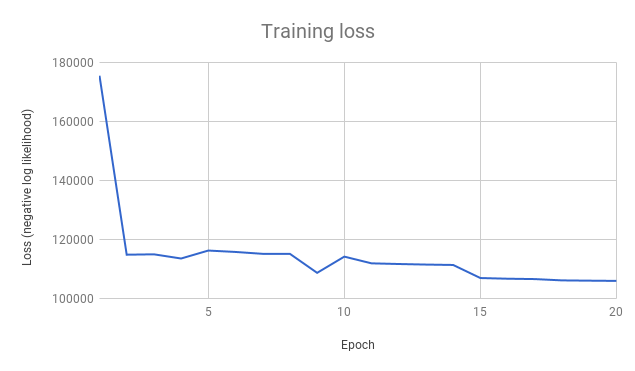
\includegraphics[scale=0.35]{training-loss}
\end{center}
\caption{Training loss for logistic regression voter model}
\label{fig:training-loss}
\end{figure}

We can see in Figure \ref{fig:training-loss} that our training loss decreases over time and converges after around 10 epochs. We saw similar loss decrease and rates of convergence for our neural network model as well.

\begin{figure}[H]
\begin{center}
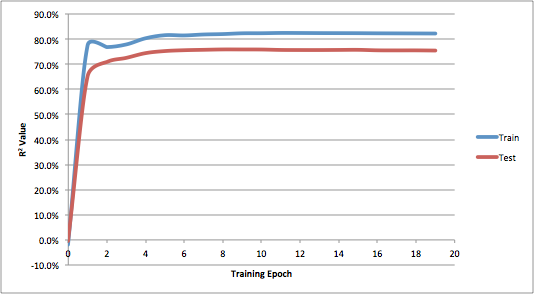
\includegraphics[scale=0.35]{holdout-R2}
\end{center}
\caption{Training and Test $R^2$ for logistic regression voter model}
\label{fig:holdout-R2}
\end{figure}

Figure \ref{fig:holdout-R2} shows model $R^2$ over time if we use logistic regression to represent individual voter behavior. The final training set $R^2$ for this model is 82.2\% and the final test set $R^2$ is 75.4\%.

\begin{figure}[H]
\begin{center}
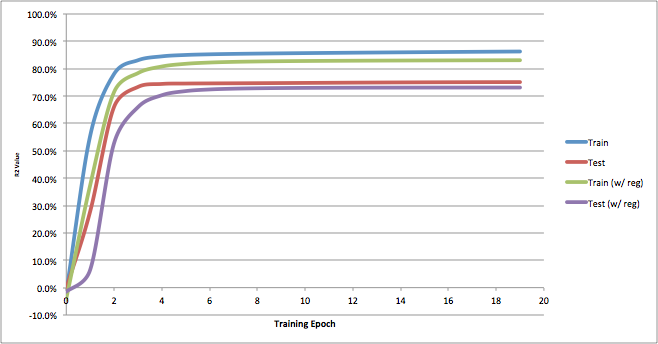
\includegraphics[scale=0.35]{holdout-R2-neural}
\end{center}
\caption{Training and Test $R^2$ for neural network voter model}
\label{fig:holdout-R2-neural}
\end{figure}

Figure \ref{fig:holdout-R2-neural} shows model $R^2$ over time if we use a neural network to represent individual voter behavior. The final training set $R^2$ for this model is 86.3\% and the final test set $R^2$ is 75.1\%. The training set accuracy is higher than in the logistic regression model, but the test set accuracy is slightly lower. The neural network's additional complexity does not seem to be helping us better model the data. We also tried adding L2 regularization by setting $\lambda = 0.7$ as well as trying some other values, but we saw no improvement to test set $R^2$.

\subsection{Weak labeling results}

After we were convinced that our model performed well at a higher level, we then wanted to show model accuracy at the individual voter level. However, due to the nature of voting data and secret ballot, we do not actually have any labeled data that we can use to validate our model. To get around this, we derived and used weak labels as an approximate way to gauge our model's performance. Weak labels have been studied in prior literature and are used in supervised learning problems where either no labeled data is available or the available data is insufficient ~\cite{rbvr2017}.

We applied two different forms of weak labels to gauge model performance at the individual voter level. First, we evaluated our model only against landslide precincts in the test set, where we define a landslide precinct to be one where 90\% or more of voters supported the same candidate. We evaluated our model against voters in these precincts and expected to see the model predicting very high probabilities of voting for Clinton for voters in precincts that actually went to Clinton and predicting very low probabilities of voting for Clinton for voters in precincts that actually went to Trump.

\begin{figure}[H]
\begin{center}
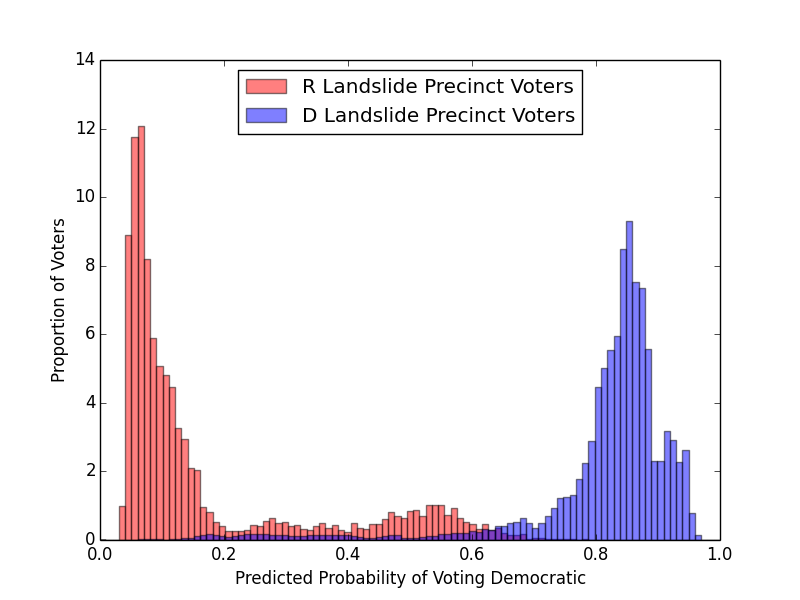
\includegraphics[scale=0.4]{lanslideHist19}
\end{center}
\caption{Predictions for voters in landslide precincts}
\label{fig:lanslideHist19}
\end{figure}

Figure \ref{fig:lanslideHist19} has the expected bimodal distribution - the voters we looked at are either heavily in favor of or heavily against Clinton, lining up with the expected results in landslide precincts.

The second form of weak labeling we looked at assumed that 2016 Republican primary voters voted for Trump in the general election while 2016 Democratic primary voters voted for Clinton in the general election. We assume that voters who voted in the primary would tend to have strong party loyalty, so we would expect to see a bimodal distribution here as well where voters were predicted to vote for either Clinton or Trump with a very high probability. We rebuilt our model but took out the features indicating whether or not voters voted in their respective primaries, and then evaluated our model only on test set voters who voted in a primary.

\begin{figure}[H]
\begin{center}
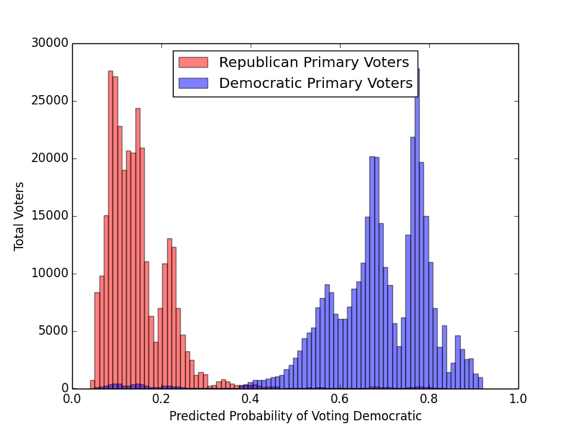
\includegraphics[scale=0.4]{primaryVoters19}
\end{center}
\caption{Predictions for primary election voters}
\label{fig:primaryVoters19}
\end{figure}

Figure \ref{fig:primaryVoters19} has the expected bimodal distribution, indicating that the model has learned that primary voters are indeed more likely to vote along party lines in the general election as well. These two weak label results show that our model does predict individual voter performance accurately.

\subsection{Final model trained on all data}

After we were convinced of the accuracy of the model, we then trained it using our entire dataset to build our final voter model. Our model coefficients are available in the below table. Note that positive values correspond to a higher probability of voting for Clinton.

\begin{table}[H]
\centering
\begin{tabular}{|l|c|}
\hline
Model Term & Value \\
\hline 
Apartment Dweller & 0.998  \\
Registered Democrat & 0.990  \\
County College Educated \% & 0.390  \\
Voted in the Democratic Primary & 0.294  \\
County Population Density & 0.204  \\
Female & 0.123  \\
County Latino \% & 0.061  \\
County Black \% & 0.001  \\
County White \% & -0.155  \\
County Income & -0.157  \\
Male & -0.332  \\
Age & -0.333  \\
Voted in the Republican Primary & -0.407  \\
Registered Republican & -1.154  \\
\hline
\end{tabular}
\label{table:coeff}
\caption{Model coefficients. Positive values correspond to a higher probability of voting for Clinton}
\end{table}

These results are in line with what we would expect. For example, older and lower income voters are more likely to vote for Trump while women and registered Democrats are more likely to vote for Clinton. These results also help show that we have developed an explanatory model for voter preference. 

\section{Conclusion and Future Work}

We have used aggregated precinct-level election data to build a model predicting how individual voters will vote by using Poisson binomial GLMs. This is not only the first time in literature that individual voter prediction models have been built without relying on polling data or other unreliable sources, but also the first time that the Poisson binomial distribution has been used as a generalized linear model as well. We train our model via gradient descent using a normal approximation of the Poisson binomial distribution that we derive (proof in the Appendix), and we validate the accuracy of the model using weak labels. We model individual voter behavior using both logistic regression as well as a simple neural network. After validating model accuracy, we retrain the model on the entire dataset to obtain our final model revealing individual voter preferences for Pennsylvania during the 2016 presidential elections. This type of model is incredibly valuable given the inherent unreliability of polling data, especially as evidenced in recent high-profile elections.

For future work, we'd like to further explore the idea of using neural networks to represent individual voter probabilities. Our investigation of neural networks yielded results that were close to the logistic regression approach. With further exploration and tuning of hyperparameters, we could likely obtain a neural network model that outperforms the linear model. We could also look at other regularization schemes such as dropout to reduce the gap between the training and test performance. In addition to investigating neural networks further we could also look at other regression models besides logistic regression to model individual voter behavior, for example the probit distribution.

We would also like to revisit the data for counties that we were not able to use for our initial analysis so we can incorporate them into the analysis as well, and develop data pipelines that would allow us to efficiently repeat this analysis on other states and elections throughout the US. 

\newpage
\onecolumn

\section*{Appendix: Lyapunov CLT Proof}

Define $d_k = \sum_{i = 1}^n d_{k, i}$ to be the number of Democratic votes in precinct $k$, where $d_{k, i}$ is an indicator variable denoting whether person $i$ in precinct $k$ voted for Clinton. $d_k$ follows a Poisson binomial distribution with success probabilities $p_k = (p_{k, 1}, \dots, p_{k, n})$. Define $s_{k}^2 = \sum_{i = 1}^{n} p_{k, i} (1-p_{k, i})$. 
We check the Lyapunov CLT \cite{billingsley1995probability} condition for the fourth moment: 

\begin{align*}
\lim_{n \to \infty} \frac{1}{s_k^4} \sum_{i = 1}^n E \left( (d_{k, i} - p_{k, i})^4 \right) &= \lim_{n \to \infty} \frac{\sum_{i = 1}^n p_{k, i}(1-p_{k, i}) \left( 3p_{k, i}^2 - 3p_{k, i} + 1 \right)}{\left(\sum_{i = 1}^n p_{k, i} \left( 1- p_{k, i} \right) \right)^2} \stackrel{?} = 0 
\end{align*}

Observe that $3p_{k, i}^2 - 3p_{k, i} + 1 \in (0, 1)$ if $p_{k, i} \in (0, 1)$. Hence, the numerator is strictly less than $\sum_{i = 1}^n p_{k, i} (1 - p_{k, i})$. Hence, if we can guarantee the numerator grows without bound, then this limit is 0 and the Lyapunov CLT applies. We can do so using a simple condition, like enforcing that there is some $\epsilon > 0$ such that $\epsilon < \bar p_i < 1- \epsilon$ for all $i$ (i.e. the mean probability of voting for Clinton in a precinct never falls below some low threshold $\epsilon$ or above some high threshold $1-\epsilon$). 

The Lypaunov CLT now tells us that: 
\[ \frac{d_k - \sum_{i = 1}^{n} p_{k, i} }{s_k} \stackrel{d} \longrightarrow N(0, 1) \] 
giving us the desired asymptotic normality. 

\section{Contributions}
Evan and Nitin both worked together to define the problem and scope it out as a Poisson GLM, and find the Pennsylvania state and OpenElections datasets. Evan wrote the majority of code for the optimization algorithm and derived the CLT proof, while Nitin wrote the majority of the report and cleaned the data to allow us to use as many counties/precincts as possible. Both Evan and Nitin reviewed each other's work in addition to the parts they lead.

{\small
\bibliographystyle{ieee}
\bibliography{csbib}
}

\end{document}
